%!TEX root = report.tex
\exercise{Principal components}
Principal component analysis can be useful for describing sets of images that have the same spatial orientation, but have different values for their pixels.
That is, they describe the same objects, using the same coordinate system, but their intensities have a different interpretation.
An example is a set of images where every image uses a different spectral band, like the \texttt{WashingtonDC\_Bandx\_564.tif} images.

In a sense, the principal component transform resembles the wavelet transform, since the processes and the goals are similar.
However, from a mathematical perspective, they seem to differ severely.

\subsection{\texttt{IPprincipalcomponents}}
Our implementation of the principal component transform is based on \cite[Sec. 11.4]{gonzalez2002digital}.
In essence, it works by first formatting all images in one matrix \(\mathbf{x}\) containing one image on every row, then retrieving the eigenvectors of the covariance matrix of \(\mathbf{x}\), arranging them by their eigenvalues in descending order in a matrix \(\mathbf{A}\), and finally multiplying \(\mathbf{A}\) with the difference matrix \(\mathbf{D} = \mathbf{x} - \mathbf{m_x}\), where \(\mathbf{m_x}\) is the mean vector of \(\mathbf{x}\).

Our implementation can be seen in the listing of the \texttt{IPprincipalcomponents} function below.
The input argument \texttt{k} can be set to use the \texttt{k} largest eigenvalues and their corresponding eigenvectors for the reconstruction of the original image.
\matlabexternal{../IPprincipalcomponents.m}

\subsection{Reading and arranging images}
\begin{figure}[htb]
 \centering
 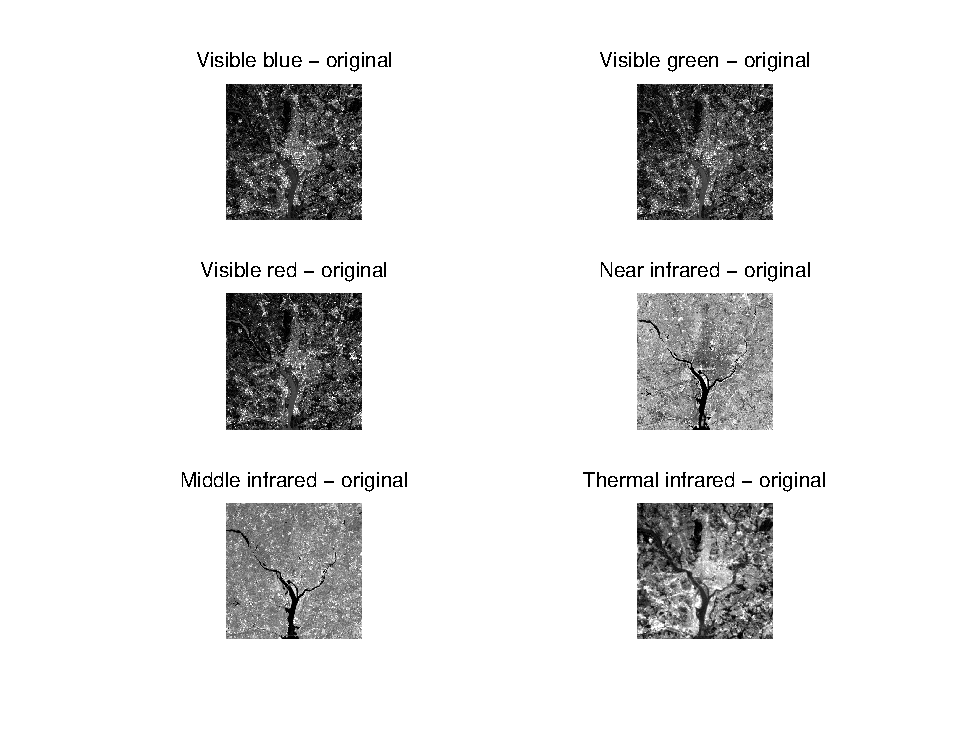
\includegraphics[width=\linewidth]{original_pca.eps}
 \caption{The original images of which the principal image components are computed}
 \label{fig:original_pca}
\end{figure}
\[
\texttt{images} = \begin{bmatrix}
	17  & 22  & \ldots & 26  & 26   \\[0.3em]
	6   & 20  & \ldots & 27  & 27   \\[0.3em]
	9   & 19  & \ldots & 28  & 28   \\[0.3em]
	154 & 98  & \ldots & 149 & 149  \\[0.3em]     
	94  & 101 & \ldots & 116 & 116  \\[0.3em]
	95  & 73  & \ldots & 84  & 84  
\end{bmatrix}
\]
The \texttt{images} does indeed contain 6 rows of the images with \(564^2\) columns.
\clearpage

\subsection{Principal components transform}
The principal component transform has been applied to the different spectral bands of the loaded images.
The results are shown in Figure~\ref{fig:full_pca}.

The eigenvalues (in descending order) are 10344, 2966, 1401, 203, 94 and 31.

\begin{figure}[htb]
 \centering
 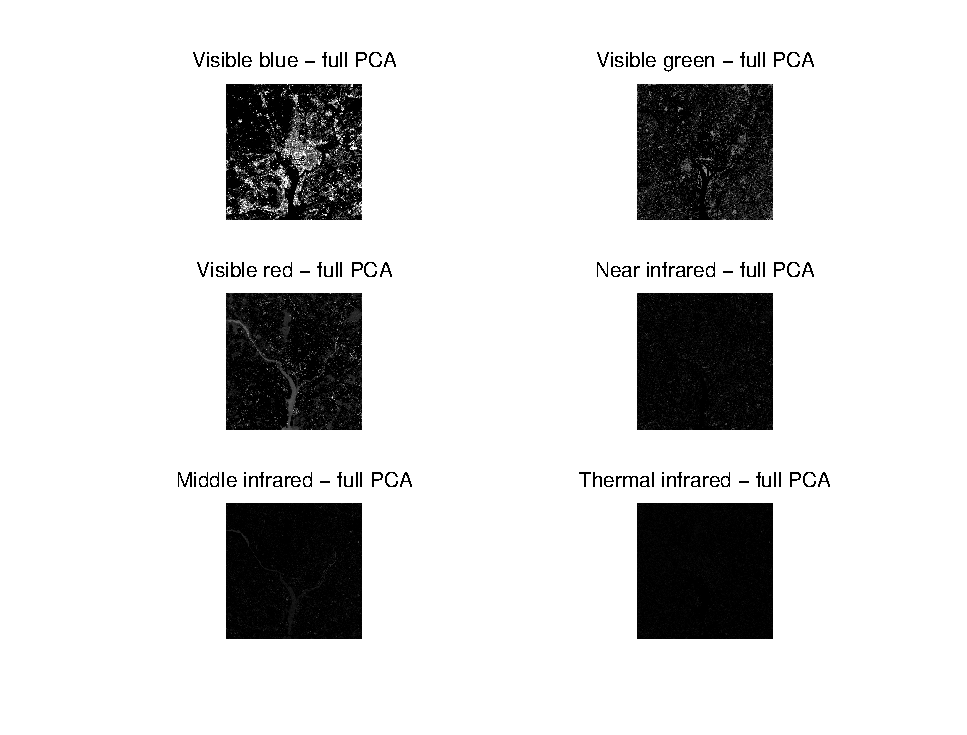
\includegraphics[width=\linewidth]{full_pca.eps}
 \caption{The principal components of the matrix constructed in (b)}
 \label{fig:full_pca}
\end{figure}

\clearpage

\subsection{Partial reconstruction}
The transformed images can be transformed back a similar version of the original images, by using the three largest eigenvalues and their corresponding eigenvectors.
The results are shown in Figure~\ref{fig:partial_recon_pca}.
The difference of the partial reconstruction is shown in Figure~\ref{fig:differences_pca}, where the sum of the differences with the original image is shown in parentheses.

\begin{figure}[htb]
 \centering
 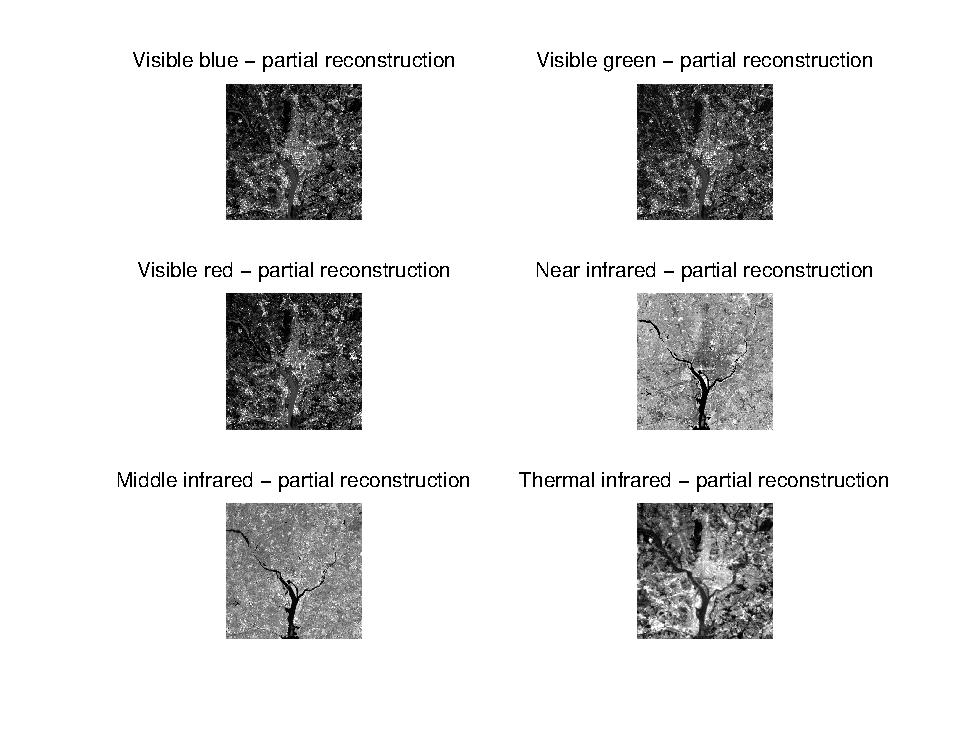
\includegraphics[width=\linewidth]{partial_recon_pca.eps}
 \caption{The reconstruction of the matrix constructed in (b) using three largest eigenvalues}
 \label{fig:partial_recon_pca}
\end{figure}

\begin{figure}[htb]
 \centering
 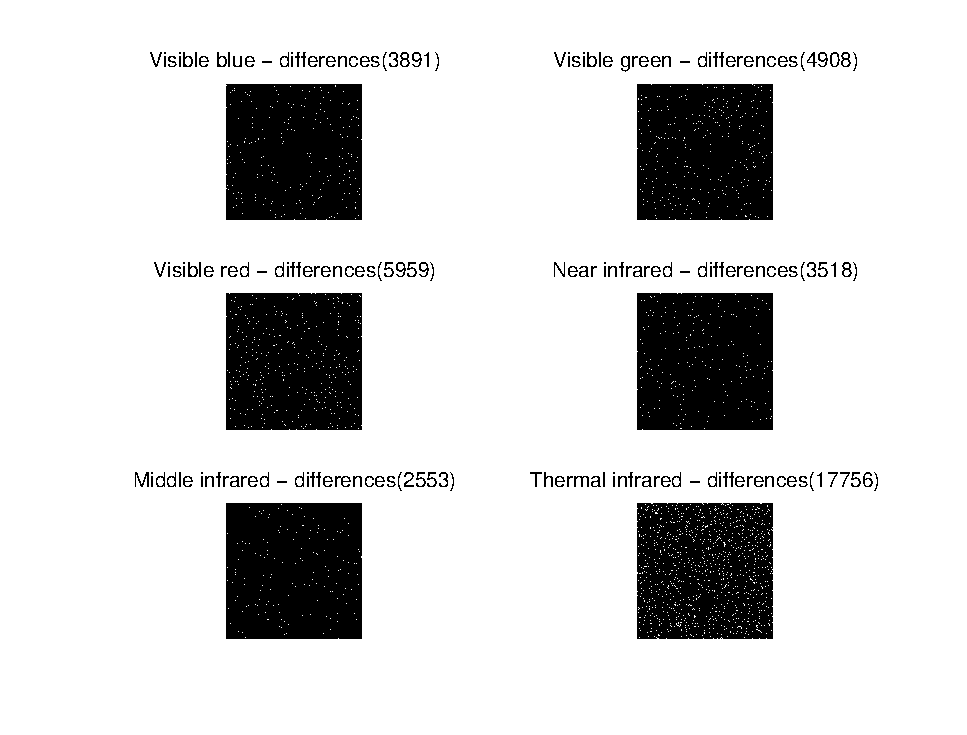
\includegraphics[width=\linewidth]{differences_pca.eps}
 \caption{Difference between the matrix constructed in (b) and the partial reconstruction using three largest eigenvalues.}
 \label{fig:differences_pca}
\end{figure}

It is visible that the partial reconstruction fails to retain all minor details that were in the original image.
This is due to the fact that only a part of the information is used.

It seems like an appropriate way to remove noise from an image, because the noise contributes in particular to the low-variation channels of the PCA. 

\clearpage